\section{Results}
\label{sec:results}
The results first describe the UNI2-h experiment on its own, with the endpoints of the Virchow2 study, and then compare the two encoders through the pre-fixed paired contrast and the six listed conclusions.

\subsection{Damage under UNI2-h}
The balanced CE model reaches 36.08 percent BA $[33.11, 39.08]$, 0.45 points below its Virchow2 counterpart. It loses $D=4.32$ points $[2.48, 6.17]$ at $\rho=50$ and $5.97$ points $[4.13, 7.97]$ at $\rho=100$; at native shares the damage of $0.72$ points $[-0.46, 1.91]$ cannot be distinguished from zero. All three damages lie within about one point of the Virchow2 values (3.54, 4.95, and 0.85). As under Virchow2, the LoRA damage at $\rho=100$ is smaller than the frozen readout's 7.19 points, and again because of the balanced model: LoRA's 36.08 percent stays 2.15 points below the frozen UNI2-h readout's 38.23 percent, while the imbalanced LoRA model (30.11 percent) lands within one point of the frozen value implied by its damage (31.04 percent). These frozen values come from different draws and are descriptive.

\subsection{Recovery per method}
Figure~\ref{fig:recovery} and Table~\ref{tab:recovery} give each method's paired recovery under UNI2-h. At $\rho=100$, six of eight variants recover a material part of the damage, the same six as under Virchow2: CUDA (2.75 points $[1.47, 4.12]$), classifier-only and end-to-end GCL (2.39 and 2.34), train-time and post-hoc logit adjustment (2.28 and 2.04), and balanced sampling (2.03). cRT (0.74) and DisAlign (0.23) again recover a positive amount below the one-point threshold. CUDA's share of the damage, 0.46 $[0.26, 0.71]$, is the largest, followed by the two GCL forms at 0.40 and 0.39. No share interval reaches 1, and at $\rho=100$ no method formally reaches full recovery: CUDA's accuracy interval, $[30.45, 35.42]$, ends below the balanced 36.08 percent.

At $\rho=50$, CUDA (2.05 points, share 0.47), end-to-end and classifier-only GCL (1.96 and 1.78), post-hoc logit adjustment (1.50), and balanced sampling (1.22, interval $[0.09, 2.42]$) recover a material part. Train-time logit adjustment gains 1.09 points with an interval that just touches zero, $[-0.01, 2.25]$. CUDA and both GCL forms formally reach full recovery at $\rho=50$, but their paired shares, with intervals ending below 0.80, show that the gap is not closed. At native shares, seven of eight recoveries lie between $-0.65$ and $0.36$ points with intervals that include zero. CUDA gains 0.95 points $[0.09, 1.91]$, just below the one-point threshold, and reaches 36.31 percent, above the balanced CE model.

\begin{figure}[t]
  \centering
  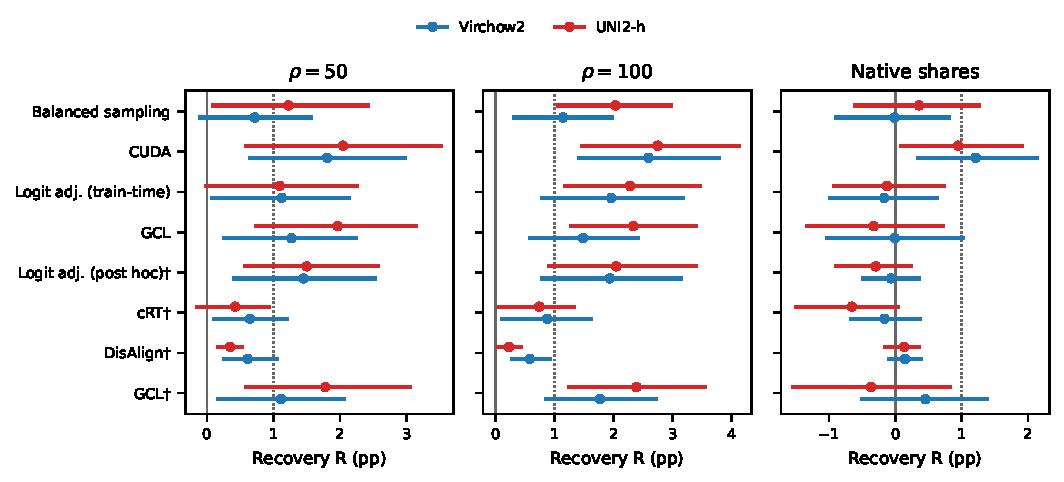
\includegraphics[width=\textwidth]{fig_recovery.pdf}
  \caption{Under both encoders, CUDA, GCL, and logit adjustment recover one to three points at $\rho=50$ and $\rho=100$, and at native shares no method except CUDA moves. Paired recovery $R_m$ with 95\% intervals for Virchow2 (blue) and UNI2-h (red); the solid line marks zero and the dotted line the one-point threshold. $^{\dagger}$Classifier only.}
  \label{fig:recovery}
\end{figure}

\begin{table}[t]
\centering
\footnotesize
\setlength{\tabcolsep}{3.5pt}
\resizebox{\textwidth}{!}{%
\begin{tabular}{@{}lccccc@{}}
\toprule
& \multicolumn{2}{c}{$\rho=50$ ($D=4.32$)} & \multicolumn{2}{c}{$\rho=100$ ($D=5.97$)} & N ($D=0.72$) \\
\cmidrule(lr){2-3}\cmidrule(lr){4-5}\cmidrule(lr){6-6}
Method & $R_m$ & share & $R_m$ & share & $R_m$ \\
\midrule
CUDA & \textbf{2.05} $[0.59, 3.52]$ & 0.47 $[0.17, 0.79]$ & \textbf{2.75} $[1.47, 4.12]$ & 0.46 $[0.26, 0.71]$ & 0.95 $[0.09, 1.91]$ \\
GCL$^{\dagger}$ & \textbf{1.78} $[0.59, 3.05]$ & 0.41 $[0.18, 0.63]$ & \textbf{2.39} $[1.25, 3.55]$ & 0.40 $[0.23, 0.59]$ & $-0.37$ $[-1.54, 0.83]$ \\
GCL & \textbf{1.96} $[0.74, 3.15]$ & 0.46 $[0.24, 0.69]$ & \textbf{2.34} $[1.28, 3.39]$ & 0.39 $[0.23, 0.60]$ & $-0.33$ $[-1.33, 0.73]$ \\
Logit adj.\ (train-time) & 1.09 $[-0.01, 2.25]$ & 0.25 $[-0.00, 0.44]$ & \textbf{2.28} $[1.18, 3.47]$ & 0.38 $[0.23, 0.55]$ & $-0.13$ $[-0.93, 0.73]$ \\
Logit adj.\ (post hoc)$^{\dagger}$ & \textbf{1.50} $[0.57, 2.57]$ & 0.35 $[0.17, 0.53]$ & \textbf{2.04} $[0.91, 3.39]$ & 0.34 $[0.19, 0.49]$ & $-0.29$ $[-0.90, 0.23]$ \\
Balanced sampling & \textbf{1.22} $[0.09, 2.42]$ & 0.28 $[0.03, 0.49]$ & \textbf{2.03} $[1.07, 2.98]$ & 0.34 $[0.20, 0.49]$ & $0.36$ $[-0.61, 1.26]$ \\
cRT$^{\dagger}$ & 0.42 $[-0.15, 0.94]$ & 0.10 $[-0.04, 0.21]$ & 0.74 $[0.07, 1.33]$ & 0.12 $[0.01, 0.21]$ & $-0.65$ $[-1.50, 0.04]$ \\
DisAlign$^{\dagger}$ & 0.35 $[0.17, 0.53]$ & 0.08 $[0.04, 0.14]$ & 0.23 $[0.05, 0.44]$ & 0.04 $[0.01, 0.07]$ & $0.13$ $[-0.15, 0.35]$ \\
\bottomrule
\end{tabular}}
\caption{Under UNI2-h, six variants recover at least one point at $\rho=100$, and no share interval reaches the full damage. Recovery $R_m$ in BA points and share of the CE damage, with paired 95\% intervals; bold marks material recovery ($R_m\geq1$, interval above zero). $^{\dagger}$Classifier only, frozen encoder; unmarked rows train end to end. Shares at native shares are omitted because the damage there cannot be distinguished from zero.}
\label{tab:recovery}
\end{table}

\subsection{Imbalance-specific recovery}
The balanced gains repeat the Virchow2 pattern with smaller or equal magnitudes (Table~\ref{tab:specific}). CUDA improves the balanced model by $G=1.04$ points, with an interval that now just includes zero, $[-0.04, 1.96]$. cRT loses 0.53 points $[-1.06, -0.02]$, the two GCL forms lose 0.36 and 0.79 points with intervals that include zero, and DisAlign is indistinguishable from CE.

Net of these gains, classifier-only GCL corrects 3.18 points $[1.74, 4.62]$ of the damage at $\rho=100$, a share of 0.53 $[0.33, 0.77]$, and end-to-end GCL 2.69 points; both are again the largest imbalance-specific recoveries. cRT's 1.28 points $[0.38, 2.09]$ remain material. CUDA's imbalance-specific recovery, 1.71 points $[0.23, 3.45]$ or a share of 0.29, becomes material under UNI2-h, whereas under Virchow2 its interval included zero (1.20 points $[-0.16, 2.62]$). At $\rho=50$ only the two GCL forms are material (2.57 and 2.32 points); CUDA (1.01, interval $[-0.59, 2.87]$) and cRT (0.96) fall short. At native shares every imbalance-specific recovery lies within half a point of zero.

\begin{table}[t]
\centering
\small
\resizebox{\textwidth}{!}{%
\begin{tabular}{@{}lccccc@{}}
\toprule
& & \multicolumn{3}{c}{$R_m-G_m$} & $\rho=100$ \\
\cmidrule(lr){3-5}\cmidrule(lr){6-6}
Method & $G_m$ & $\rho=50$ & $\rho=100$ & N & share \\
\midrule
CUDA & 1.04 $[-0.04, 1.96]$ & 1.01 $[-0.59, 2.87]$ & \textbf{1.71} $[0.23, 3.45]$ & $-0.09$ $[-1.31, 1.29]$ & 0.29 $[0.04, 0.54]$ \\
GCL & $-0.36$ $[-1.27, 0.51]$ & \textbf{2.32} $[1.05, 3.71]$ & \textbf{2.69} $[1.43, 4.00]$ & 0.03 $[-1.17, 1.32]$ & 0.45 $[0.25, 0.71]$ \\
GCL$^{\dagger}$ & $-0.79$ $[-1.77, 0.17]$ & \textbf{2.57} $[1.09, 4.12]$ & \textbf{3.18} $[1.74, 4.62]$ & 0.42 $[-1.14, 1.91]$ & 0.53 $[0.33, 0.77]$ \\
cRT$^{\dagger}$ & $-0.53$ $[-1.06, -0.02]$ & 0.96 $[0.15, 1.67]$ & \textbf{1.28} $[0.38, 2.09]$ & $-0.12$ $[-1.23, 0.78]$ & 0.21 $[0.07, 0.34]$ \\
DisAlign$^{\dagger}$ & $-0.01$ $[-0.06, 0.03]$ & 0.36 $[0.17, 0.56]$ & 0.25 $[0.06, 0.45]$ & 0.15 $[-0.14, 0.39]$ & 0.04 $[0.01, 0.08]$ \\
\bottomrule
\end{tabular}}
\caption{Under UNI2-h, classifier-only GCL again corrects the largest part of the imbalance, and CUDA's imbalance-specific recovery is material at $\rho=100$. Balanced gain $G_m$ and imbalance-specific recovery $R_m-G_m$ (Eq.~\ref{eq:endpoints}) in BA points, with its share of the CE damage at $\rho=100$; paired 95\% intervals, bold marks material recovery. $^{\dagger}$Classifier only. Balanced sampling and logit adjustment have $G_m=0$ by construction.}
\label{tab:specific}
\end{table}

\subsection{Encoder contrast}
No quantity meets the pre-fixed rule for encoder dependence at any allocation. Table~\ref{tab:contrast} lists the paired contrasts at $\rho=100$, and Figure~\ref{fig:contrast} shows $\delta R_m$ for all three imbalanced allocations. The largest point contrast at $\rho=100$ is the damage itself: UNI2-h loses 1.02 points more than Virchow2, but the interval, $[-0.29, 2.48]$, includes zero. Five of the eight recoveries are larger under UNI2-h in point estimate, by up to 0.89 points (balanced sampling) and 0.85 points (end-to-end GCL), which is consistent with a somewhat larger damage to recover; none of these intervals excludes zero. The only intervals that exclude zero belong to DisAlign, whose recovery and imbalance-specific recovery are 0.35 and 0.34 points smaller under UNI2-h, well below the one-point threshold. The balanced gains differ by at most 0.36 points. At $\rho=50$ and at native shares no $|\delta|$ exceeds 0.82 points, and no interval excludes zero.

\begin{table}[t]
\centering
\small
\begin{tabular}{@{}llccc@{}}
\toprule
Quantity & Method & Virchow2 & UNI2-h & $\delta$ (UNI2-h $-$ Virchow2) \\
\midrule
$\mathrm{BA}(\mathrm{CE},1)$ & -- & 36.53 & 36.08 & $-0.45$ $[-2.13, 1.21]$ \\
$D_{100}$ & -- & 4.95 & 5.97 & $1.02$ $[-0.29, 2.48]$ \\
\midrule
$R_m$ & CUDA & 2.59 & 2.75 & $0.16$ $[-1.13, 1.63]$ \\
 & Logit adj.\ (train-time) & 1.96 & 2.28 & $0.32$ $[-0.89, 1.56]$ \\
 & Logit adj.\ (post hoc)$^{\dagger}$ & 1.94 & 2.04 & $0.11$ $[-0.67, 0.96]$ \\
 & GCL & 1.48 & 2.34 & $0.85$ $[-0.32, 2.09]$ \\
 & GCL$^{\dagger}$ & 1.77 & 2.39 & $0.62$ $[-0.50, 1.67]$ \\
 & Balanced sampling & 1.14 & 2.03 & $0.89$ $[-0.17, 1.93]$ \\
 & cRT$^{\dagger}$ & 0.88 & 0.74 & $-0.14$ $[-0.92, 0.55]$ \\
 & DisAlign$^{\dagger}$ & 0.58 & 0.23 & $-0.35$ $[-0.67, -0.08]$ \\
\midrule
$G_m$ & CUDA & 1.39 & 1.04 & $-0.36$ $[-1.93, 1.12]$ \\
 & GCL & $-0.33$ & $-0.36$ & $-0.03$ $[-1.19, 1.23]$ \\
 & GCL$^{\dagger}$ & $-0.64$ & $-0.79$ & $-0.15$ $[-1.48, 1.31]$ \\
 & cRT$^{\dagger}$ & $-0.48$ & $-0.53$ & $-0.06$ $[-0.71, 0.65]$ \\
 & DisAlign$^{\dagger}$ & $-0.01$ & $-0.01$ & $-0.00$ $[-0.06, 0.06]$ \\
\midrule
$R_m-G_m$ & CUDA & 1.20 & 1.71 & $0.51$ $[-1.34, 2.52]$ \\
 & GCL & 1.81 & 2.69 & $0.88$ $[-0.67, 2.60]$ \\
 & GCL$^{\dagger}$ & 2.41 & 3.18 & $0.77$ $[-0.91, 2.36]$ \\
 & cRT$^{\dagger}$ & 1.36 & 1.28 & $-0.08$ $[-1.28, 0.92]$ \\
 & DisAlign$^{\dagger}$ & 0.59 & 0.25 & $-0.34$ $[-0.67, -0.07]$ \\
\bottomrule
\end{tabular}
\caption{No paired encoder contrast at $\rho=100$ excludes zero with a size of at least one point. Point estimates per encoder in BA points and the paired contrast $\delta$ (Eq.~\ref{eq:delta}) with its 95\% interval. $^{\dagger}$Classifier only.}
\label{tab:contrast}
\end{table}

\begin{figure}[t]
  \centering
  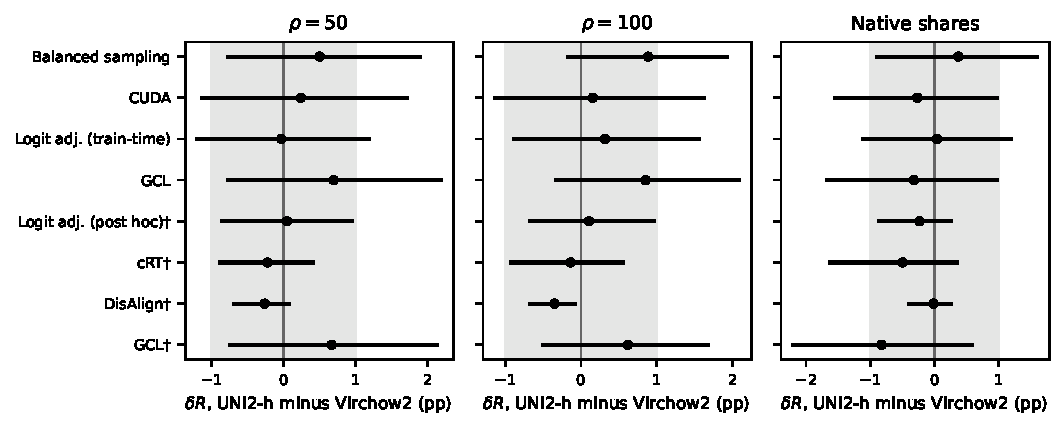
\includegraphics[width=\textwidth]{fig_contrast.pdf}
  \caption{Every paired recovery contrast overlaps zero or stays inside the one-point band. Paired contrast $\delta R_m$ (UNI2-h minus Virchow2) with 95\% intervals; the grey band marks $\pm1$ point. $^{\dagger}$Classifier only.}
  \label{fig:contrast}
\end{figure}

The descriptive summaries point the same way under imbalance. At $\rho=100$ all eight material-recovery verdicts agree between encoders, and the Spearman correlation of $R_m$ across the eight variants is 0.81. At $\rho=50$ the correlation is 0.83 and six of eight verdicts agree; the two that differ sit at the threshold, balanced sampling (material only under UNI2-h, lower bound 0.09) and train-time logit adjustment (material only under Virchow2, lower bound $-0.01$ under UNI2-h). At native shares the correlation drops to 0.33 and seven verdicts agree, the exception being CUDA (1.21 points under Virchow2, 0.95 under UNI2-h). There, all recoveries but CUDA's are indistinguishable from zero under both encoders, so their ranking is dominated by noise.

\subsection{Conclusions of the Virchow2 study}
Table~\ref{tab:claims} checks the six conclusions listed in advance. Four carry over to UNI2-h. CUDA again gives the largest recovery at $\rho=100$, although its lead over the next method shrinks from 0.63 to 0.36 points, and differences between methods are not tested. Logit adjustment remains the only method that substantially lifts tail recall (Section~\ref{sec:rank}). No share interval reaches 1, and the LoRA model on the balanced allocation stays below the frozen readout. Two conclusions weaken. CUDA's imbalance-specific recovery is material under UNI2-h; classifier-only GCL and cRT remain material, so the conclusion fails only in its CUDA part. Its contrast with Virchow2, 0.51 points $[-1.34, 2.52]$, is not resolved, so the verdict changes because an estimate near the threshold moved, not because the encoders demonstrably differ. Classifier-only methods recover as much as end-to-end ones within the matched pairs: post-hoc logit adjustment trails its train-time form by 0.24 points, and classifier-only GCL exceeds end-to-end GCL by 0.05 points. As a family they recover less: excluding CUDA, the mean share at $\rho=100$ is 0.37 for the end-to-end and 0.23 for the classifier-only methods, against 0.31 and 0.26 under Virchow2. The gap widens because balanced sampling gains under UNI2-h while DisAlign and cRT recover little. These family and pair comparisons are point estimates without intervals.

\begin{table}[t]
\centering
\small
\renewcommand{\arraystretch}{1.15}
\begin{tabularx}{\textwidth}{@{}>{\raggedright\arraybackslash}p{0.27\textwidth}YY>{\raggedright\arraybackslash}p{0.12\textwidth}@{}}
\toprule
Conclusion at $\rho=100$ & Virchow2 & UNI2-h & Verdict \\
\midrule
(i) CUDA gives the largest $R_m$ & 2.59; next 1.96 & 2.75; next 2.39 (GCL$^{\dagger}$) & Holds \\
(ii) Only logit adjustment lifts tail recall substantially & Tail 5.1 to 20.2 and 22.3; others $\leq$11.9 & Tail 2.7 to 15.3 and 19.0; others $\leq$9.6 & Holds \\
(iii) No share interval reaches 1 & Highest upper bound 0.82 & Highest upper bound 0.71 & Holds \\
(iv) CUDA's $R_m-G_m$ not material; GCL$^{\dagger}$ and cRT$^{\dagger}$ material & 1.20 $[-0.16, 2.62]$; 2.41 and 1.36 material & 1.71 $[0.23, 3.45]$; 3.18 and 1.28 material & Fails for CUDA \\
(v) Classifier-only recovers as much as end-to-end & Mean share without CUDA 0.31 vs.\ 0.26 & Mean share without CUDA 0.37 vs.\ 0.23; pairs within 0.24 & Pairs only \\
(vi) LoRA balanced model below frozen readout & 36.53 vs.\ 39.57 & 36.08 vs.\ 38.23 & Holds \\
\bottomrule
\end{tabularx}
\caption{Four of the six pre-listed conclusions carry over to UNI2-h, and the two that weaken do so without a resolved encoder contrast. Values in BA points, recall points, or shares; tail recall is the patient-macro recall of the rarest third of classes for CE and the two logit-adjustment forms. The frozen readouts in (vi) come from different draws and are descriptive. $^{\dagger}$Classifier only.}
\label{tab:claims}
\end{table}

\subsection{Where recovery lands}
\label{sec:rank}
Under UNI2-h, the CE model at $\rho=100$ keeps 2.7 percent recall in the tail third of classes by assigned rank, against 33.9 percent when balanced, and gains 16.6 points in the head (Figure~\ref{fig:rank}). Logit adjustment raises the tail to 15.3 (train-time) and 19.0 percent (post hoc), at a cost of six to nine points of head recall. CUDA and the two GCL forms recover through the body instead, 36.5 to 38.2 against 25.1 percent, and raise the tail only to between 7.6 and 9.6 percent. Balanced sampling, cRT, and DisAlign leave the tail between 3.7 and 7.9 percent. Every method thus places its recovery in the same rank group as under Virchow2, while the tail recalls of CE and of logit adjustment are two to five points lower under UNI2-h. Rank-group recalls are point estimates.

\begin{figure}[t]
  \centering
  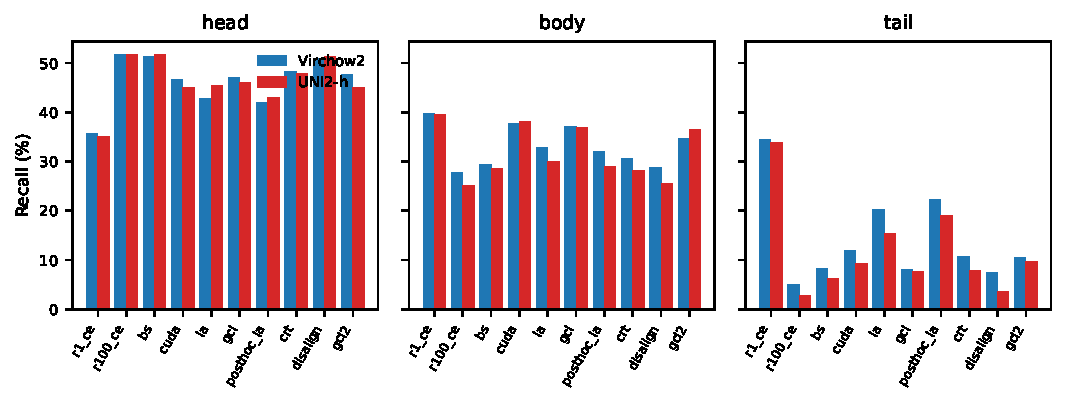
\includegraphics[width=0.85\textwidth]{fig_rank_recall.pdf}
  \caption{Under both encoders, only logit adjustment lifts tail recall substantially at $\rho=100$, and CUDA and GCL gain in the body. Patient-macro recall of the head, body, and tail thirds of classes by assigned rank, averaged over shards, for Virchow2 (blue) and UNI2-h (red). $^{\dagger}$Classifier only.}
  \label{fig:rank}
\end{figure}

\subsection{Selected strengths and probability quality}
Validation selection behaves as under Virchow2 for most methods. At $\rho=100$, train-time logit adjustment selects the full correction $\tau=1$ in 23 of 30 shards and post-hoc logit adjustment in 15, balanced sampling selects $s=1$ in 23, and GCL selects $\sigma=0.05$ in 18 (end to end) and 15 (classifier only) of 30. CUDA selects $p_{\mathrm{aug}}=1$ in 14 of 30 shards at $\rho=100$ and in 12 at $\rho=50$, never at native shares, and never on the balanced allocation, where 0.5 wins 18 shards and 0.25 wins 12. DisAlign is the exception. Under UNI2-h it selects the largest value of its grid, $\gamma=2$, in 12 of 30 shards at $\rho=100$, and $\gamma=3$, the largest value of the wider native-shares grid, in 19 of 30 shards at native shares. Under Virchow2, $\gamma=1$ or 1.5 won 22 of 30 shards at $\rho=100$. DisAlign's grid was copied unchanged by design, so under UNI2-h it may stop short of DisAlign's best strength.

Imbalance again mainly worsens raw calibration. At $\rho=100$ the CE model's raw negative log-likelihood (NLL) rises from 2.95 to 3.58 nats and its raw expected calibration error (ECE) from 31.5 to 39.8 points. CUDA has the lowest raw NLL, 2.26 nats $[2.10, 2.43]$, and raw ECE, 21.5 points $[17.8, 26.7]$, below even the balanced CE model; the two logit-adjustment forms follow (3.00 and 2.89 nats), and cRT (4.04) and end-to-end GCL (3.91) are highest. After validation temperature scaling, every method lies between 1.75 (CUDA) and 1.80 nats, around CE's 1.80 and close to the balanced 1.66, and scaled ECE ranges from 10.0 (classifier-only GCL) to 14.3 points (DisAlign) against CE's 14.1. As under Virchow2, CUDA curbs raw overconfidence, but no method improves probability quality beyond what temperature scaling already provides.

\section{Discussion}
\label{sec:discussion}
\textbf{Does mitigation under LoRA depend on the encoder?} Not measurably. None of the 20 pre-fixed contrasts per allocation meets the encoder-dependence rule, the material-recovery verdicts agree for all eight methods at $\rho=100$, and the method ranking is stable at both imbalance ratios. The two encoders also share the structure of the result: CUDA, GCL, and logit adjustment recover one to three points at $\rho=100$; GCL's classifier-only form corrects the most imbalance net of its balanced effect; logit adjustment alone restores the tail; no method closes the gap; and at native shares nothing but CUDA's general gain moves. The conclusions of the Virchow2 study \citep{queisler2026mitigationBracs} therefore do not depend on that choice of encoder.

\textbf{What do the two weakened conclusions mean?} Both reflect estimates near a threshold, not a resolved difference. CUDA's imbalance-specific recovery rises from 1.20 to 1.71 points and crosses into materiality, but the paired contrast of 0.51 points has an interval almost four points wide. Read across both encoders, CUDA's imbalance-specific part is probably positive and smaller than its recovery against CE, with its balanced gain explaining a third to a half of that recovery; whether it reaches one point is not settled by either experiment alone. The family comparison shifts because three methods moved by less than a point in opposite directions, while the matched pairs, which isolate the effect of adapting the encoder from the method itself, agree within 0.3 points under both encoders. The finding that a frozen-encoder classifier re-fit suffices for a given method holds; the family-level summary does not, because it averages over methods of very different strength.

\textbf{How large a difference could have been missed?} The paired intervals of the recovery contrasts span between about 0.6 and 3.0 points, those of the damage up to 3.2 points, and those of the imbalance-specific recoveries up to 4.2 points. An encoder difference of one point in a single method's recovery would therefore often remain unresolved, and the null result bounds encoder effects at roughly one to two points, not at zero. The point estimates do lean one way: UNI2-h's damage is one point larger, and five of eight recoveries are larger with it. A larger damage that the methods recover in proportion would produce exactly this pattern, and the shares, which differ between encoders by about 0.1 or less, support that reading.

\textbf{Does UNI2-h change the frozen-versus-LoRA picture?} No. Under both encoders, LoRA's balanced model is two to three points less accurate than the frozen readout, and the smaller LoRA damage reflects this weaker reference rather than a more robust imbalanced model. With UNI2-h, the best mitigated model at $\rho=100$, CUDA at 32.86 percent, stays 5.4 points below the frozen balanced readout, the same margin as under Virchow2. For BRACS, adapting either encoder with this recipe and then mitigating does not outperform a frozen readout trained on balanced data.

\textbf{Limitations.} The study adds a second encoder but keeps one dataset and one adaptation scheme. All settings were tuned under Virchow2 and transferred unchanged: the 600 training steps, the LoRA rank and target modules, and the strength grids. This keeps the comparison paired, but it measures each encoder under a recipe fitted to the other, and UNI2-h's lower balanced accuracy may partly reflect that. DisAlign's selections concentrate on the largest grid value under UNI2-h, so its small recovery, and the only contrasts whose intervals exclude zero, may partly reflect a truncated grid. The two encoders also differ in their pooled embedding (1,536 against 2,560 dimensions), so the contrast describes two complete encoder-plus-pooling pipelines. The comparisons with the frozen readouts use different draws and are descriptive. Imbalance-specific recovery assumes that a method's balanced effect carries over additively to the imbalanced allocations, as in the Virchow2 study.
